\section{Obiettivo}
L’obiettivo del lavoro svolto è stato quello di utilizzare dei Dataset di immagini biomedicali e sfruttarli per allenare una rete neurale convoluzionale il cui scopo è la classificazione. \\
Nel dettaglio, in una prima parte dell'esperienza è stato utilizzato un dataset di radiografie pettorali per addestrare un modello che riconoscesse quali tra i soggetti presentassero la polmonite e quali no. \\
Nella seconda parte si utilizza un dataset di risonanze magnetiche cerebrali per stimare una diagnosi dello stato del paziente tra 4 possibili situazioni: paziente sano, paziente con glioma, meningioma o tumore ipofisario. \\


\section{CNN per la rilevazione della polmonite}
\subsection{Il dataset}
Il dataset utilizzato,
 pubblicato sulla piattaforma Kaggle \footnote{Kaggle è una piattaforma online per competizioni di modelli predittivi e analitici fondata nel 2010. Ad oggi conta più di 500.000 utenti} da Paulo Breviglieri, è costituito da 5856 radiografie.
 É una versione rivisitata di un altro dataset le cui immagini sono state selezionate da uno studio di coorte retrospettivo \footnote{Uno studio di coorte prende in considerazione un gruppo di individui che presentano caratteristiche comuni (sesso, età, etnia…) e che hanno come unica differenza tra loro l’esposizione o meno al fattore di rischio. Questo tipo di studio identifica persone con una malattia (o altre variabili di interesse) e le paragona ad un gruppo di controllo appropriato che non presenti la patologia.

 Questo gruppo viene osservato per un periodo di tempo prestabilito, al termine del quale si analizzerà la presenza o meno dell’esito atteso.} di pazienti pediatrici di età che va da 1 a 5 anni di un centro medico di Canton (Hong Kong). Le radiografie sono state realizzate come quadro clinico di routine per i pazienti. Le immagini stesse sono state sottoposte a screening per il controllo della qualità e tutte quelle illeggibili sono state rimosse. Le diagnosi sono poi state confermate da due fisici esperti e successivamente da un terzo specialista prima di essere utilizzate per allenare sistemi di AI. \\
 Il modello di CNN utilizzato dovrà essere in grado di riconoscere i pattern di immagine tipici della malattia. L’identificazione è infatti talvolta complicata anche per i medici più esperti. \\
Sotto: esempio illustrativo di raggi-X in pazienti con polmonite. 
\begin{figure}[hb!]
\begin{subfigure}{.32\textwidth}
  \centering
  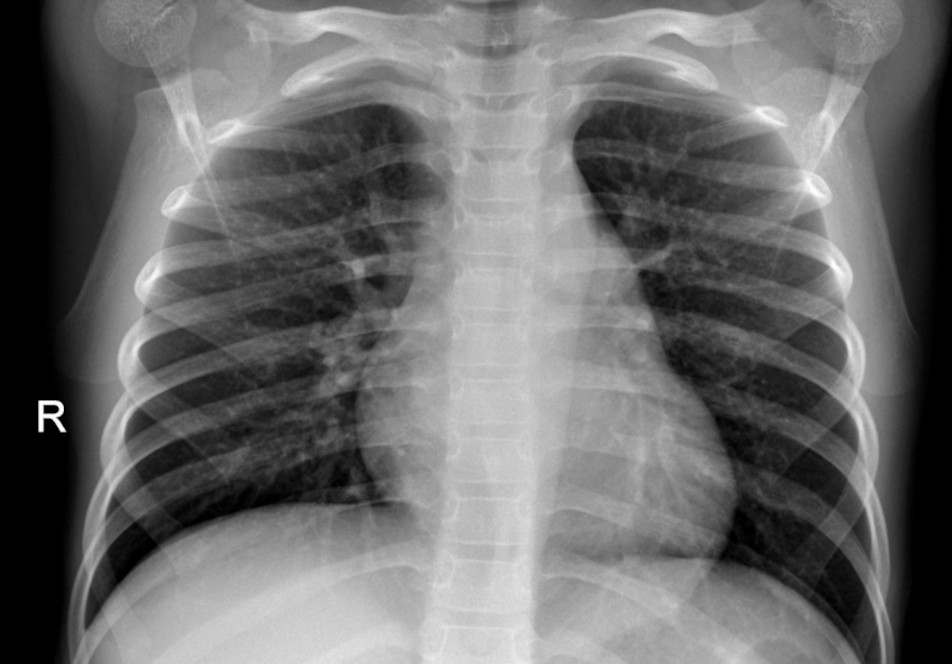
\includegraphics[width=.95\linewidth]{san}
  %\caption{1a}
  \caption{}
  \label{fig:snap1}
\end{subfigure}%
\begin{subfigure}{.32\textwidth}
  \centering
  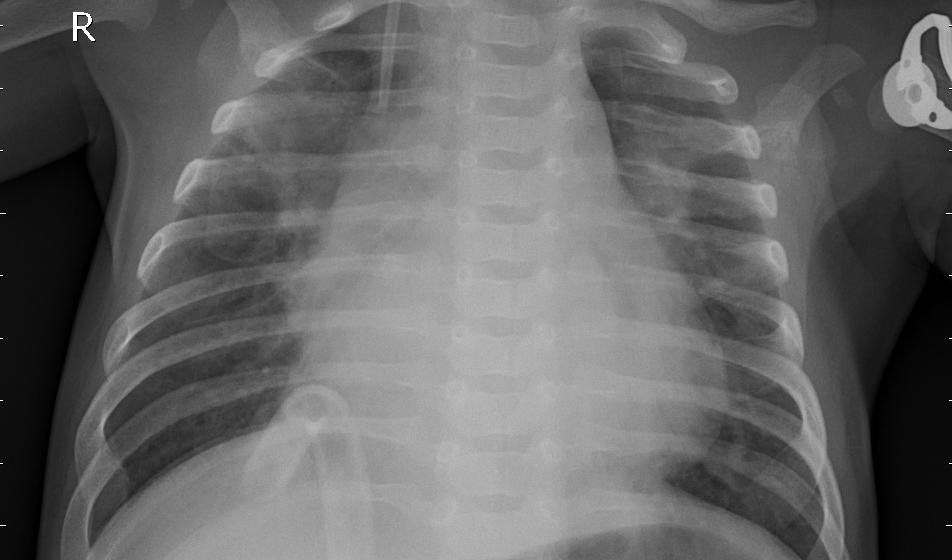
\includegraphics[width=.95\linewidth]{bacteria}
  %\caption{1a}
  \caption{}
  \label{fig:snap2}
\end{subfigure}%
\begin{subfigure}{.32\textwidth}
  \centering
  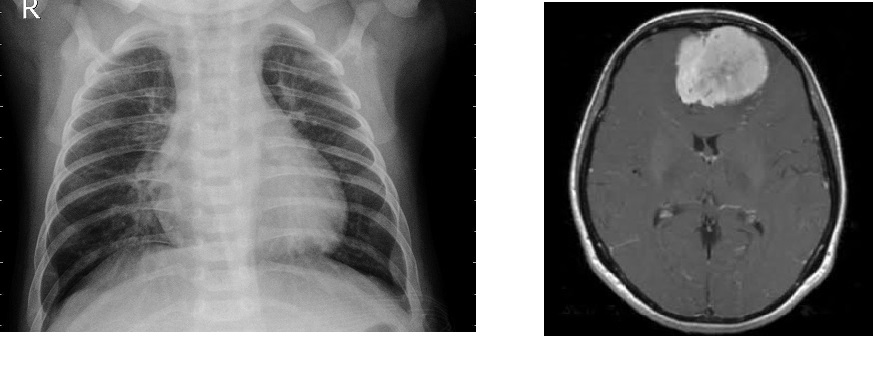
\includegraphics[width=.95\linewidth]{virus}
  %\caption{1b}
  \caption{}
  \label{fig:snap3}
\end{subfigure}
\caption{Si può notare come un soggetto sano (a) mostri polmoni senza aree di anormale opacità. L’immagine (b) è invece un caso di polmonite batterica che presenta il tipico consolidamento. (c) è un caso di polmonite virale che presenta un pattern interstiziale più diffuso in entrambi i polmoni.}
\label{fig:fig}
\end{figure} 

Il dataset è organizzato in 3 cartelle: una di Training (per l'addestramento stesso della rete), una di Testing (per testare le capacità di generalizzazione della rete) e una di Validation (per testare la bontà della rete e rilevare overfitting e/o underfitting in fase di addestramento). Ognuna di esse è organizzata così: 
\begin{itemize}
    \item 4,192 immagini per il training (1,082 casi normali, 3,110 di polmonite) 
    \item 1,040 immagini di validation (267 casi normali, 773 di polmonite) 
    \item 624 immagini per il testing (234 casi normali, 390 di polmonite) 
\end{itemize}
Il numero di immagini è sufficientemente grande per poter essere utilizzato per gli obiettivi preposti ricorrendo alle tecniche di deep learning per la computer vision di ambito biomedico. \\
Le proporzioni del dataset rispettano ampiamente gli standard che di solito si utilizzano per addestrare un modello di classificazione: un set di testing e uno di validation che è sono circa il (10-20)\% del totale, il resto è lasciato al training.
Si va adesso a sintetizzare quali sono stati i principali passaggi per l’implementazione della CNN.

\subsection{Setup iniziale}
Il primo step per realizzare il classificatore è l’importazione delle librerie necessarie per la manipolazione di tensori, per le operazioni matematiche e per la relizzazione di grafici (Pandas, NumPy, MatPlotLib), così come librerie di Keras per l’image preprocessing e oggetti di Deep Learning, tra cui:
\begin{itemize}
\item \lstinline{Sequential}, classe di Keras che permette di raggruppare layers, che non sono altro che i blocchi di base per la costruzione delle reti neurali, in uno stack lineare e realizzare così un oggetto di classe \lstinline{Model}, che è implementato in modo tale da riuscire a elaborare deduzioni una volta superata la fase di training; 
\item \lstinline{Conv2D}, classe che realizza la convoluzione spaziale sulle immagini 2D. Questo strato sfrutta un kernel di convoluzione il quale è coinvolto con lo strato in input per produrre un tensore in output. Se questo strato è usato per primo nel modello è necessario inserire come parametro la tupla rappresentante le dimensioni delle immagini in input. In questo strato è possibile scegliere il numero e le dimensioni del filtro, il valore dello stride (s=1 di default), il tipo di padding e altri parametri del caso; 
\item \lstinline{MaxPool2D}, realizza l’operazione di pooling, dunque è possibile anche qui scegliere la dimensione della pool, il valore dello stride, il tipo di padding...;
\item \lstinline{Flatten}, classe che permette di trasformare la feature map allo strato precedente in un vettore che viene dato in input alla ANN in seguito;
\item \lstinline{Dense}, classe che implementa un regolare strato di una NN. In sostanza è questo lo strato che implementa la somma pesata degli input con i pesi e il bias di cui si parlava nel capitolo 1. 
\end{itemize}

\subsection{Definizione degli iperparametri}
Successivamente sono stati fissati dei valori per gli iperparametri, ovvero quelle variabili poste all'inizio del codice, prima che il processo di apprendimento cominci. I valori degli iperparametri sono davvero importanti per l’accuratezza del modello e delle predizioni, infatti sono stati fatti variare alcune volte prima di arrivare alla migliore soluzione. I principali sono: 
\begin{itemize}
\item Le dimensioni di input dell’immagine, perchè è necessario che durante la fase di training vi sia un'uniformità delle dimensioni degli input;
\item il numero di epoche, cioè il numero di volte in cui l’algoritmo di apprendimento lavora sull’intero dataset prima di procedere con l’aggiornamento dei pesi. Sulla base di queste varia anche la durata dell’apprendimento. Infatti gli step di apprendimento per epoca sono pari alla divisione tra il numero di istanze del set di trainig e la batch size;
\item la batch size: è un iperparametro dell’algoritmo del gradiente discendente che indica il numero di campioni di training sui quali lavorare prima che venga fatto un aggiornamento dei pesi. Sia in questa esperienza sia in quella successiva si utilizza un algoritmo di apprendimento in modalità \emph{mini-batch} in quanto il dataset è abbastanza numeroso, ovvero si utilizza un valore di batch più grande rispetto a 1, così che non si vada ad aggiornare i valori dei pesi ogni volta che il sistema riceve un campione in input, quindi più del necessario, ottimizzando la durata dell'epoca e quindi del training. Di norma la batch size deve essere un valore che sia divisore del numero totale di immagini del dataset e nelle folders. 
\item il numero di feature maps: più che ne sono più caratteristiche differenti si possono andare a scovare ma allo stesso tempo aumenta anche il numero di parametri e se si vuole evitare il rischio di overfitting occorre aumentare la complessità del modello.
\item il numero di canali d'immagine utilizzati nel processo di learning: per le immagini RGB colorate tale parametro è pari a 3, mentre nel caso di immagini in scala di grigi vale 1. In tale caso le immagini sono digitali RGB ma vedremo che utilizzare solo un canale è la soluzione che porta ad una maggiore accuratezza.
\end{itemize}

Facendo riferimento agli iperparametri utilizzati per la costruzione del classificatore sono stati
 scelti tali iperparametri come i migliori per questa esperienza:\\
\lstinline{img_height = img_width = 600}\\
\lstinline{epochs = 10}\\
\lstinline{batch_size = 8}\\
\lstinline{hyper_featuremaps = 32}\\
\lstinline{hyper_channels = 1}\\
\lstinline{hyper_mode = 'grayscale'}\\

E’ stata utilizzata una dimensione per le immagini di 600 x 600 pixel associata a una batch size di 8
 affinchè lo spazio occupato in RAM non sia eccessivamente alto.  \\

\subsection{Definizione e compilazione del modello}
Per questa esperienza è stato utilizzato un modello di rete neurale convoluzionale semplice, che consiste di questi strati:\\
\begin{itemize}
\item 5 strati di Convoluzione/pooling: i primi 3 producono ognuno 32 feature maps con la convoluzione, 
generanti ognuna una feature map di pooling, per gli ultimi 2 sono stati invece utilizzati 64 filtri, 
così da produrre 64 feature maps anch’esse seguite da un’operazione di pooling. La convoluzione è stata performata
 con dei kernel di dimensione 3x3 e con una funzione di attivazione non lineare, cioè la ReLu. Nel capitolo precedente
  è stato indicato in parte il perchè questo tipo di funzione è quella maggiormente utilizzata in ambito di
   classificazione d’immagine, in quanto risolve in parte il problema della scomparsa del gradiente, uno dei 
   principali problemi del deep learning. Durante la fase di backpropagation i pesi degli strati in
    prossimità dell’input restano costanti o si aggiornano molto lentamente al contrario di quanto 
    accade per gli strati vicini all’output. Questo può provocare un rallentamento della rete ed è dovuto 
    alle funzioni di attivazione. Funzioni di attivazione come la sigmoide infatti sono funzioni a codominio
     limitato e hanno una derivata
      che presenta una regione di significatività piuttosto piccola, oltre la quale il valore della derivata stessa
       è molto piccolo. Per la regola della catena nella fase di backpropagation è necessario andare a fare un
        prodotto di derivate che è pari al numero di strati della rete neurale. A mano a mano che però si torna 
        indietro dall’output verso l’input però, moltiplicando valori molto vicini allo zero tra di loro si
         ottengono valori di aggiornamento dei pesi infinitesimi che comportano l'impossibilità per la rete
          di aggiornare i pesi correttamente, soprattutto quando si vanno ad utilizzare reti con più di due strati, e quindi quelle tipiche del deep learning.
           L'operazione di Max-pooling viene fatta con delle pool di dimensione
           2x2. Lo stride è stato lasciato quello di default a 1 e il padding scelto è il ‘same’, affinchè la
            dimensione dell’input sia uguale alla dimensione dell’output. 
\item Strato di flattening: necessario per introdurre la successiva ANN, connessa all’ultimo strato
 di pooling tramite un unico tensore unidimensionale.
\item 3 di strati completamente connessi rispettivamente di 128, 64 e 1 neuroni. 
L’ultimo strato consta di un solo neurone in quanto la classificazione è binaria. 
\end{itemize}

Tipicamente si parte sempre dall’utilizzare un numero di filtri più piccolo, come in questo caso 32,
 per poi andare ad aumentare a multipli di questa dimensione. 
Il modello è infine compilato usando il metodo \lstinline{compile()} usando la funzione di ottimizzazione Adam, 
algoritmo che si
 basa sull’idea del gradiente discendente ma che però elabora una stima adattativa dei momenti 
 del primo e del secondo ordine, permettendo una maggiore efficienza rispetto agli altri algoritmi
  a livello di costo computazionale per il training, a discapito di una conseguente minor capacità
   di generalizzazione. Inoltre Adam adatta il learning rate a seconda dei vari strati anche sulla base
    di quello che è il problema della scomparsa del gradiente di cui si è parlato sopra. \\
In fase di compilazione si sceglie anche la metrica, che permette di calcolare quanto spesso le label effettive
 coincidono con
 le predizioni fatte ed è dunque un parametro necessario per monitorare l’accuratezza e l’errore del modello.
  Una metrica di questo tipo viene settata col nome di \lstinline{'accuracy'}. 
  Per il calcolo dell’errore si usa una funzione di costo che in questo caso è chiamata \emph{binary crossentropy},
   (funzione di entropia incrociata binaria) poichè si va a fare una classificazione binaria.\\


   
    
\begin{python} %se voglio dividere in due pagine metto due \begin pyton separati
cnn = Sequential()
cnn.add(Conv2D(hyper_featuremaps, (3, 3), activation="relu", input_shape=(img_width, img_height, hyper_channels)))
cnn.add(MaxPooling2D(pool_size = (2, 2)))
cnn.add(Conv2D(hyper_featuremaps, (3, 3), activation="relu", input_shape=(img_width, img_height, hyper_channels)))
cnn.add(MaxPooling2D(pool_size = (2, 2)))
cnn.add(Conv2D(hyper_featuremaps, (3, 3), activation="relu", input_shape=(img_width, img_height, hyper_channels)))
cnn.add(MaxPooling2D(pool_size = (2, 2)))
cnn.add(Conv2D(hyper_featuremaps * 2, (3, 3), activation="relu", input_shape=(img_width, img_height, hyper_channels)))
cnn.add(MaxPooling2D(pool_size = (2, 2)))
cnn.add(Conv2D(hyper_featuremaps * 2, (3, 3), activation="relu", input_shape=(img_width, img_height, hyper_channels)))
cnn.add(MaxPooling2D(pool_size = (2, 2)))
cnn.add(Flatten())
cnn.add(Dense(activation = 'relu', units = 128))
cnn.add(Dense(activation = 'relu', units = 64))
cnn.add(Dense(activation = 'sigmoid', units = 1))
cnn.compile(optimizer = 'adam', loss = 'binary_crossentropy', metrics = ['accuracy'])
cnn.summary()

\end{python}
\begin{lstlisting}[caption= {Modello in Python utilizzato} ]
\end{lstlisting}

\newpage

\begin{python}
    Model: "sequential_1"
_________________________________________________________________
Layer (type)                 Output Shape              Param #   
=================================================================
conv2d_5 (Conv2D)            (None, 498, 498, 32)      320       
_________________________________________________________________
max_pooling2d_5 (MaxPooling2 (None, 249, 249, 32)      0         
_________________________________________________________________
conv2d_6 (Conv2D)            (None, 247, 247, 32)      9248      
_________________________________________________________________
max_pooling2d_6 (MaxPooling2 (None, 123, 123, 32)      0         
_________________________________________________________________
conv2d_7 (Conv2D)            (None, 121, 121, 32)      9248      
_________________________________________________________________
max_pooling2d_7 (MaxPooling2 (None, 60, 60, 32)        0         
_________________________________________________________________
conv2d_8 (Conv2D)            (None, 58, 58, 64)        18496     
_________________________________________________________________
max_pooling2d_8 (MaxPooling2 (None, 29, 29, 64)        0         
_________________________________________________________________
conv2d_9 (Conv2D)            (None, 27, 27, 64)        36928     
_________________________________________________________________
max_pooling2d_9 (MaxPooling2 (None, 13, 13, 64)        0         
_________________________________________________________________
flatten_1 (Flatten)          (None, 10816)             0         
_________________________________________________________________
dense_3 (Dense)              (None, 128)               1384576   
_________________________________________________________________
dense_4 (Dense)              (None, 64)                8256      
_________________________________________________________________
dense_5 (Dense)              (None, 1)                 65        
=================================================================
Total params: 1,467,137
Trainable params: 1,467,137
Non-trainable params: 0

\end{python}
\begin{lstlisting}[caption = {Riepilogo del modello. La colonna \lstinline{layer} indica il tipo di strato di cui si tratta. La colonna output mostra la tupla con le dimensioni dello strato in uscita, con una dimensione
    in più \lstinline{None} che è aggiunta per ospitare la batch size. La terza colonna \lstinline{Param \#} indica il numero di pesi all'interno della rete, i quali possono essere distinti in addestrabili, cioè quelli che vengono aggiornati durante la fase di backpropagation, e quelli per cui questo non vale per motivi di regolarizzazione della rete. Il numero totale di parametri si trova \lstinline{(kernel_height*kernel_width*input_filters*output_filters) + 
    output_filters}. Ad esempio nel primo strato si avra 3*3*32*1+32=320.}]
  
\end{lstlisting}

\subsection{Creazione dei set di training e validation traminte l’uso dell’image flowing}
Tramite l’utilizzo della classe di Keras  \lstinline{ImageDataGenerator()} è possibile andare a caricare le
 immagini di training, testing e validation andando a richiamare su tali generatori il metodo  
 \lstinline{flowFromDirectory()} che è in grado di ritornare un oggetto di tipo DataFrameGenerator
 costituito da una tupla (X , y) dove X è un NumPy array contenente un numero di immagini pari alla 
   \lstinline{batch size} e della dimensione pari a  \lstinline{image_width}x\lstinline{image_height}indicata e 
   y è anch’esso
    un NumPy array che però contiene le label corrispondenti alle immagini prodotte. L’utilizzo di
     questa funzione è possibie perchè il dataset è strutturato in partenza in un dataset di trainining, 
     validation e testing. Inoltre tale funzione genera i set provvedendo a fare uno shuffle di tutte le immagini
      sia di training sia di  validation, mentre per il set di testing è stato inserito  \lstinline{Shuffle = False}
       così da poter testare la capacità di generalizzazione della rete e confrontare le predizioni con i risultati 
       effettivi. \\
 \lstinline{ImageDataGenarator} è una classe che permette anche di utilizzare tecniche di \emph{augmentation}
  per ampliare il dataset. Tali tecniche prevedono di andare a costruire versioni modificate delle immagini stesse. 
  Infatti il dataset, pur essendo numeroso, non lo è al punto tale da rendere sufficientemente buona l’esperienza
   di image processing. Questa mancanza può essere pertanto colmata andando ad ampliare il dataset con immagini
    che possano arricchire l’esperienza di training del modello. Tali immagini possono essere modificate in vari
     modi, ma non tutti questi sono utili nel caso di interesse: infatti alcune tecniche possono generare rumore 
     aggiuntivo e ‘’confondere’’ il sistema nella ricerca dei pattern per la rilevazione della polmonite.
     Infatti è differente classificare immagini biomedicali come i raggi
     X per capire se vi è o meno una polmonite rispetto ad una classificazione di immagini come quelli di 
     cani o di gatti. Infatti, mentre un gatto può essere visto da varie angolazioni e ciò può essere
      utile al fine di distinguerlo da un cane, operare una rotazione troppo elevata per andare a riconoscere 
      l’opacità dei polmoni in un’immagine a raggi X, non va ad arricchire il dataset, ma può portare
       addirittura a un peggioramento dell’accuratezza del modello. Nell’esperienza è stato fatto un
        training del modello dapprima senza l’utilizzo di tecniche di image augmentation, per poi confrontarlo
         con un altro training in cui è stato ampliato il dataset. \\

      Occorre pertanto scegliere accuratamente quali parametri inserire. Le tecniche che sono risultate essere utili in questo caso sono:
      \begin{itemize}
        \item \textbf{Rescaling}: dato che è stata definita la modalità di colorazione 'grayscale' ogni pixel di 
        ogni immagine avrà un valore che sta nel range [0,255] che con questa tecnica diviene compreso tra 0 e 1. 
        Un primo beneficio è che così tutte le immagini vengono trattate alla stessa maniera. 
        Infatti è possibile che alcune immagini abbiano un range alto di valori dei pixel, altre più basso,
         ma entrambe condividono poi lo stesso modello e learning rate per il training. 
        In generale è bene fare in modo che il range di valori sia compreso tra 0 e 1 così che ogni immagine
         contribuisca nella maniera più uniforme possibile per il calcolo della funzione di perdita totale e 
         quindi per l'aggiornamento dei pesi. 
        \item \textbf{Rotazione}: è stato appurato che un piccolo range di rotazione per le immagini possa essere
         utile a migliorare le capacità di generalizzazione del sistema, proprio perchè molto spesso nella pratica clinica
         le radiografie possono essere lievemente ruotate a causa dei movimenti del paziente. Il range utilizzato in questo caso è tra i 
         -5$^\circ$  e i 5$^\circ$.
         \item \textbf{Zoom}: come nel caso della rotazione, è prassi che vi siano immagini in cui il torace del paziente sia posizionato
         più o meno vicino al dispositivo che elabora l'immagine. Quindi un piccolo range di variazione dello zoom delle immagini (in questo caso è stato scelto 0.1) 
         può essere utile. 
        
      \end{itemize}


      
      \begin{figure}[H]
        \centering
        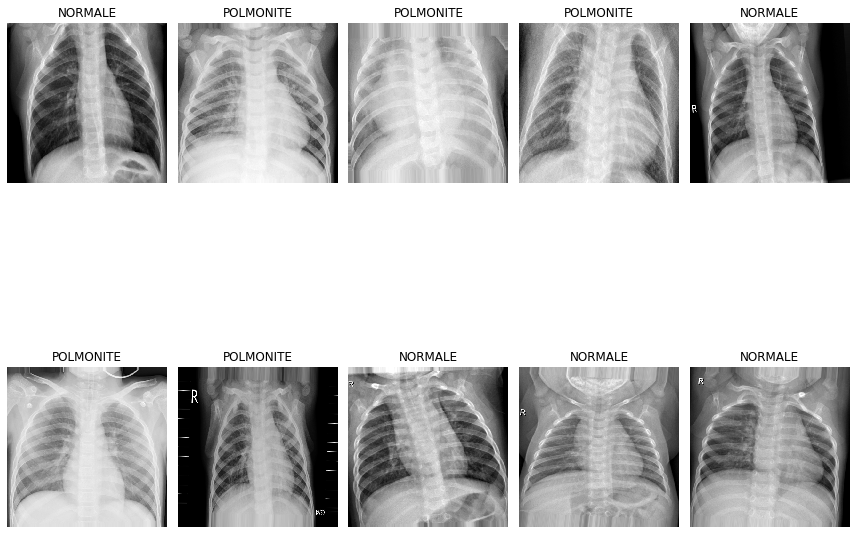
\includegraphics[width=0.9\textwidth]{Figures/best-augmented-images-pneumonia.png}
        \caption{\small{
        Campioni di immagini del dataset di training sui quali sono state aggiunte le tecniche sopra citate.
        } % end small
        } % end caption
        \label{fi:dcalc}
    \end{figure}
      
     
\subsection{Fase di fitting}
Dopo aver compilato e configurato il modello si passa alla fase di \emph{fitting}, cioè la fase di addestramento
 vera e propria. Il modello viene dunque allenato tramite le immagini del set di training, con un aggiornamento
  dei pesi che viene fatto per ogni gruppo di campioni pari alla \lstinline{batchsize}. Il set di training viene rivisto
   per un totale di 20 epoche, anche se dopo 10 la capacità di training risulta essere stagnante.
    Una volta captato questo è stata usata la funzione di callback \lstinline{EarlyStopping()} che ha fermato il
     training non appena risultava esserci overfitting. 
   Il metodo  \lstinline{fit()} ci permette anche di scegliere l’insieme di validation su cui la rete 
   può generalizzare. Ciò fa sì che non solo si possa monitorare l'accuratezza nel training, ma anche la
    capacità di generalizzazione della rete, cercando di capire se questa sta andando in overfitting, 
    underfitting o se il trade-off tra le due è accettabile, così da agire di conseguenza 
    per poterla migliorare. Si può anche definire una lista di chiamate (callbacks) per 
    customizzare il training, come definire un checkpoint dove salvare il modello così 
    da poterlo utilizzare successivamente per elaborare nuove predizioni,
     senza necessità di allenarlo nuovamente.  Inoltre è stata utilizzata una funzione che riduce il 
     valore del learning rate del 30\% automaticamente ogni due epoche in quanto molto spesso 
     il modello beneficia di ciò se l’apprendimento stagna. 
     %(Aprire parentesi nei capitoli precedenti di come il lr influenza l’apprendimento)
In questo caso il modello è stato allenato sull’insieme di training e validation definito dal dataset stesso.
 Il set di testing è l’insieme di immagini sulle quali si va a fare la valutazione finale.
  \begin{figure}[H]
    \begin{subfigure}{0.55\textwidth}
      \centering
      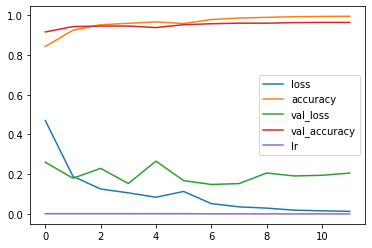
\includegraphics[width=0.95\linewidth]{Figures/history-pneumonia-no-aug.png}
      %\caption{1a}
      \caption{}
      \label{fig:snap1}
    \end{subfigure}%
    \begin{subfigure}{0.55\textwidth}
      \centering
      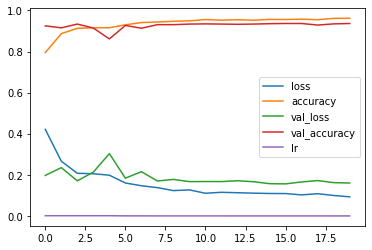
\includegraphics[width=.95\linewidth]{Figures/history-pneumonia-aug.png}
      %\caption{1a}
      \caption{}
      \label{fig:snap2}
    \end{subfigure}%
    \caption{In entrambe le figure è possibile osservare la curva ROC sul training e sul set di validation. Lo scopo è quello che la curva arancione tenda ad un gradino di ampiezza unitaria.}
    \label{fig:fig}
\end{figure} 
Alla fine si ottengono questi risultati andando a richiamare \lstinline{cnn.evaluate(test)}:
\begin{itemize}
  \item Per il caso senza modifiche al set di training risulta che l'accuracy sul training è pari al (99.61 $\pm$ 0.01)\% e quella sull'insieme di validation è del (94.44 $\pm$ 0.01)\%.
  \item  Per il caso con le modifiche al set di training risulta che l'accuracy sul training è pari al (96.99 $\pm$ 0.01)\% e quella sull'insieme di validation è del (94.61 $\pm$ 0.01)\%.
  
\end{itemize}


\subsection{Predizioni}
Infine occorre osservare come il sistema riesce a generalizzare sull’insieme di test. 
Dato che la funzione di attivazione dello strato finale del modello è la sigmoide, 
il valore dell’output starà in un range compreso tra 0 e 1 corrispondente alla probabilità che l’immagine
 su cui è stata fatta la predizione presenti polmonite o meno. 
Se si vogliono quantificare i falsi positivi e i falsi negativi occorre vedere se l’output della 
rete è superiore o inferiore a 0.5  e di conseguenza predire se si tratta di polmonite o meno.
 É possibile visualizzare la matrice di confusione\footnote{É un modo per visualizzare in maniera 
 diretta il numero di predizioni corrette/falsi-negativi/falsi-positivi}. 
 Le tabelle 5.1 e 5.2 rappresentano dei report di classificazione in cui è possibile osservare 3 diverse voci:
\begin{itemize}
  \item Precision = (Predizioni corrette) / (Predizioni corrette + Falsi positivi)
  \item Recall = Predizioni corrette / (Predizioni corrette + Falsi negativi)
  \item F1 = (2 * Precision * Recall) / (Precision + Recall)
\end{itemize}
  % Please add the following required packages to your document preamble:
% 



  \begin{table}[hb!]
  \begin{tabular}{@{}l|llll@{}}
    \toprule
                     & \textbf{precision} & \textbf{recall} & \textbf{f1-score} & \textbf{support} \\ \midrule
  \textbf{NORMALE}   & 0.99               & 0.36            & 0.53              & 234              \\
  \textbf{POLMONITE} & 0.72               & 1.00            & 0.84              & 390              \\ \midrule
  accuracy           &                    &                 & 0.76              & 624              \\
  macro avg          & 0.85               & 0.68            & 0.68              & 624              \\
  weighted avg       & 0.82               & 0.76            & 0.72              & 624              \\ \bottomrule
  \end{tabular}
  \caption{}
\end{table} 
  
  

\begin{table}[hb!]
  \begin{tabular}{@{}l|llll@{}}
  \toprule
                     & \textbf{precision} & \textbf{recall} & \textbf{f1-score} & \textbf{support} \\ \midrule
  \textbf{NORMALE}   & 0.97               & 0.85            & 0.90              & 234              \\
  \textbf{POLMONITE} & 0.91               & 0.98            & 0.95              & 390              \\ \midrule
  accuracy           &                    &                 & 0.93              & 624              \\
  macro avg          & 0.94               & 0.92            & 0.93              & 624              \\
  weighted avg       & 0.94               & 0.93            & 0.93              & 624              \\ \bottomrule
  \end{tabular}
  \caption{}
\end{table}

In sintesi l'accuratezza del modello sull'insieme di test vale:
\begin{itemize}
  \item  (75.80 $\pm$ 0.01)\% nella prima esperienza;
  \item  (93.27 $\pm$ 0.01)\% nella seconda.
\end{itemize}
Dunque sembra che, nonostante nella prima esperienza si abbia ottenuto un'accuratezza migliore sul training, 
poi le capacità di generalizzazione sono migliori quelle ottenute con la seconda.
 Ciò significa che nel primo training si è avuto un problema di overfitting. 


 \begin{figure}[H]
        \begin{subfigure}{0.55\textwidth}
          \centering
          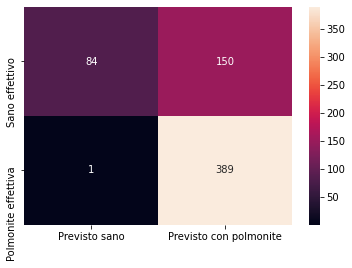
\includegraphics[width=0.95\linewidth]{Figures/conf-matrix-no-aug.png}
          %\caption{1a}
          \caption{}
          \label{fig:snap1}
        \end{subfigure}%
        \begin{subfigure}{0.55\textwidth}
          \centering
          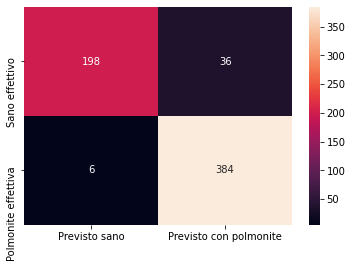
\includegraphics[width=.95\linewidth]{Figures/conf-matrix-pneumonia-aug.png}
          %\caption{1a}
          \caption{}
          \label{fig:snap2}
        \end{subfigure}%
        \caption{ Matrici di confusione ottenute. (a) è la matrice di confusione del modello con il set di
         training lasciato come l'originale. 
        Si può vedere che vi sono molti errori nel prevedere il soggetto sano. \\
        (b) è la matrice di confusione con il set di training modificato come nella Figura 5.2. 
        In questo caso vi sono pochissimi errori di predizione.
        }
        \label{fig:fig}
\end{figure} 


\begin{figure}[H]
  \centering
  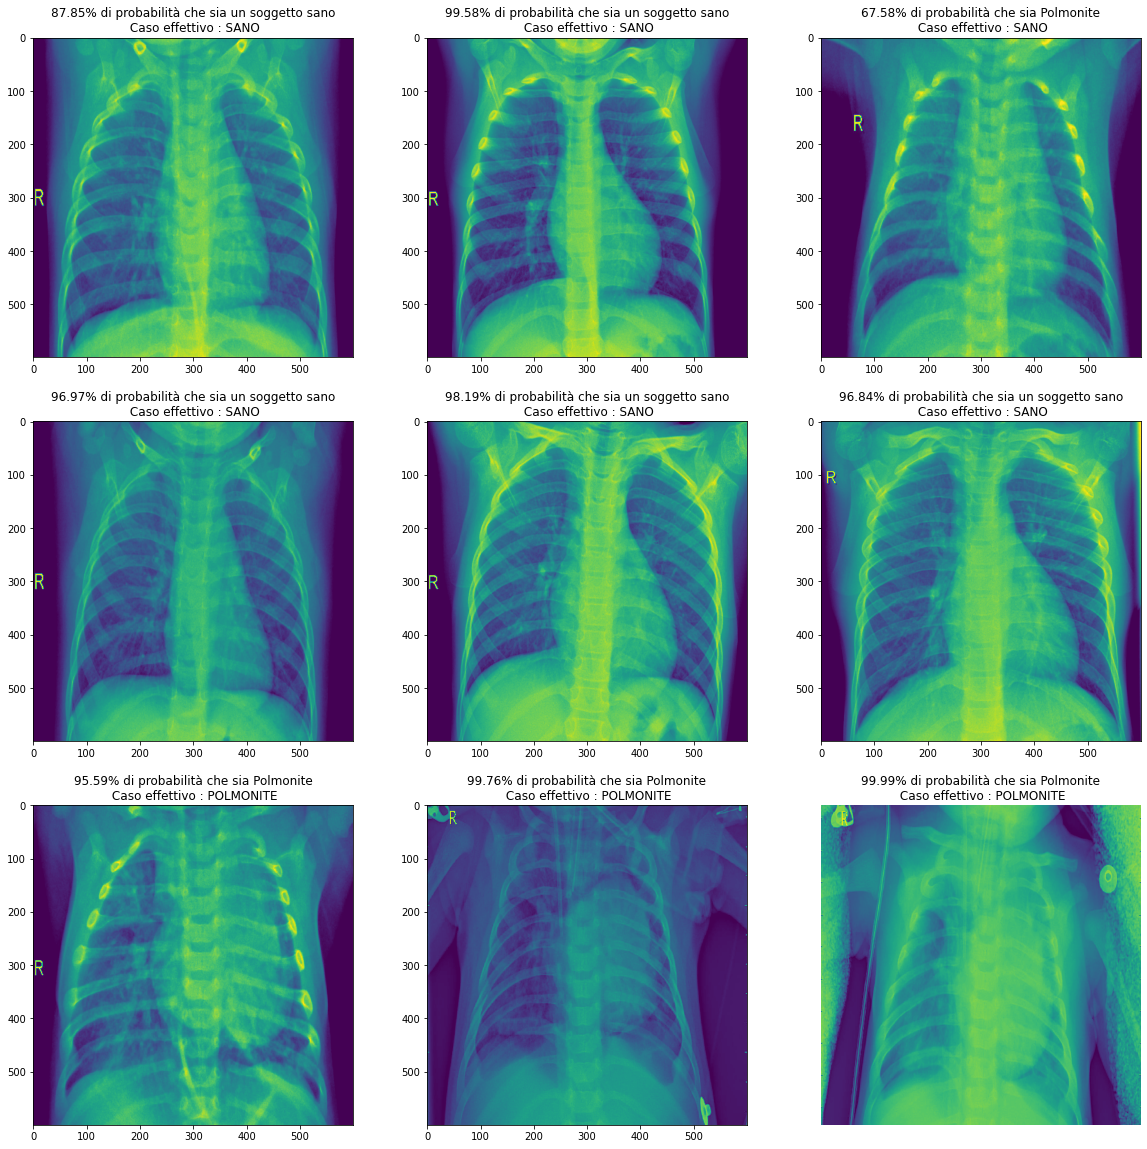
\includegraphics[width=0.9\textwidth]{Figures/test-results-pneumonia-600.png}
  \caption{\small{Dimostrazione di alcune previsioni.
  } % end small
  } % end caption
  \label{fi:dcalc}
\end{figure}
 
 
 
\subsection{Considerazioni finali}
La rete addestrata con il dataset ampliato risulta produrre buoni risultati. 
In prima istanza sicuramente grazie all’accuratezza del dataset, ma anche grazie a degli iperparametri ben scelti. 
Sono state in effetti fatte delle prove con image size di dimensioni 400x400, 500x500, 600x600 e batch size = 8, 16, 32 ,
 ma la migliore accuratezza di generalizzazione si ha con gli iperparametri della sezione 5.2.3. Risultati ragionevoli 
 sono stati trovati dopo 10 epoche, anche se è stato fatto un addestramento anche con 25 e 50 epoche
 , ma ciò risultava inutile in quanto dalla decima epoca in poi l’accuratezza 
 del modello rimane costante e non migliora. Per evitare ciò è stato utilizzato l’Early Stopping che ha
  appunto fermato il modello intorno alla decima epoca. 
Inoltre è stato provato anche ad aumentare il numero dei canali d’immagine
 da 1 a 3 ma ciò non ha fatto altro che peggiorare le prestazioni. Probabilmente 
 ciò è dovuto al fatto che per rilevare una polmonite la scala di grigi evidenzia maggiormente l’opacità del polmone. 
Sicuramente se il classificatore dovesse essere utilizzato in uno studio radiologico,
 sarebbe un buon mezzo di supporto in quanto il numero di falsi negativi è minore rispetto
  a quello dei falsi positivi ed è molto piccolo (clinicamente è meglio che sia diagnosticato 
  un falso positivo piuttosto che un falso negativo!). Sotto si mostrano i risultati ottenuti con iperparametri
   differenti (eccetto il numero di epoche in tutti i casi pari a 20), con le modifiche apportate al set di training della sezione 5.2.5
    e che hanno portato alla scelta di quelli alla sezione 5.2.3.

    \begin{table}[hb!]
      \begin{tabular}{l|lll}
      \hline
                                                                                                         & \multicolumn{1}{l|}{\textbf{training accuracy}} & \multicolumn{1}{l|}{\textbf{validation accuracy}} & \textbf{test accuracy} \\ \hline
      \textbf{\begin{tabular}[c]{@{}l@{}}batch = 16\\ image size = 500x500\\ channels = 1\end{tabular}}  & 95.99\%                                         & 93.65\%                                           & 91.98\%                \\ \hline
      \textbf{\begin{tabular}[c]{@{}l@{}}batch = 32\\ image size = 400x400\\ channels = 1\end{tabular}}  & 95.94\%                                         & 95.00\%                                           & 91.5\%                 \\ \hline
      \textbf{\begin{tabular}[c]{@{}l@{}}batch = 8\\ image size = 600 x 600\\ channels = 1\end{tabular}} & 96.49\%                                         & 94.61\%                                           & 93.26\%                \\ \hline
      \textbf{\begin{tabular}[c]{@{}l@{}}batch = 8\\ image size = 600 x 600\\ channels = 3\end{tabular}} & 96.32\%                                         & 93.94\%                                           & 92.62\%                \\ \hline
      \end{tabular}
      \end{table}
\newpage
\section{CNN per la classificazione di risonanze magnetiche cerebrali}


